%!TEX root = ../../master.tex

\section*{Votiee}
Votiee was primarily used in the first module of the course, due to the distribution between presentations and hands-on work. Votiee is a simple voting platform, where the students are provided a code that they have to input at votiee.com in order to participate in the vote. Votiee was used as a small break during the presentations, for the students to reflect upon the topic. Further Votiee was used to collect data about e.g. the students gender and ages. The data collection and answers to the questions can be found below. \\

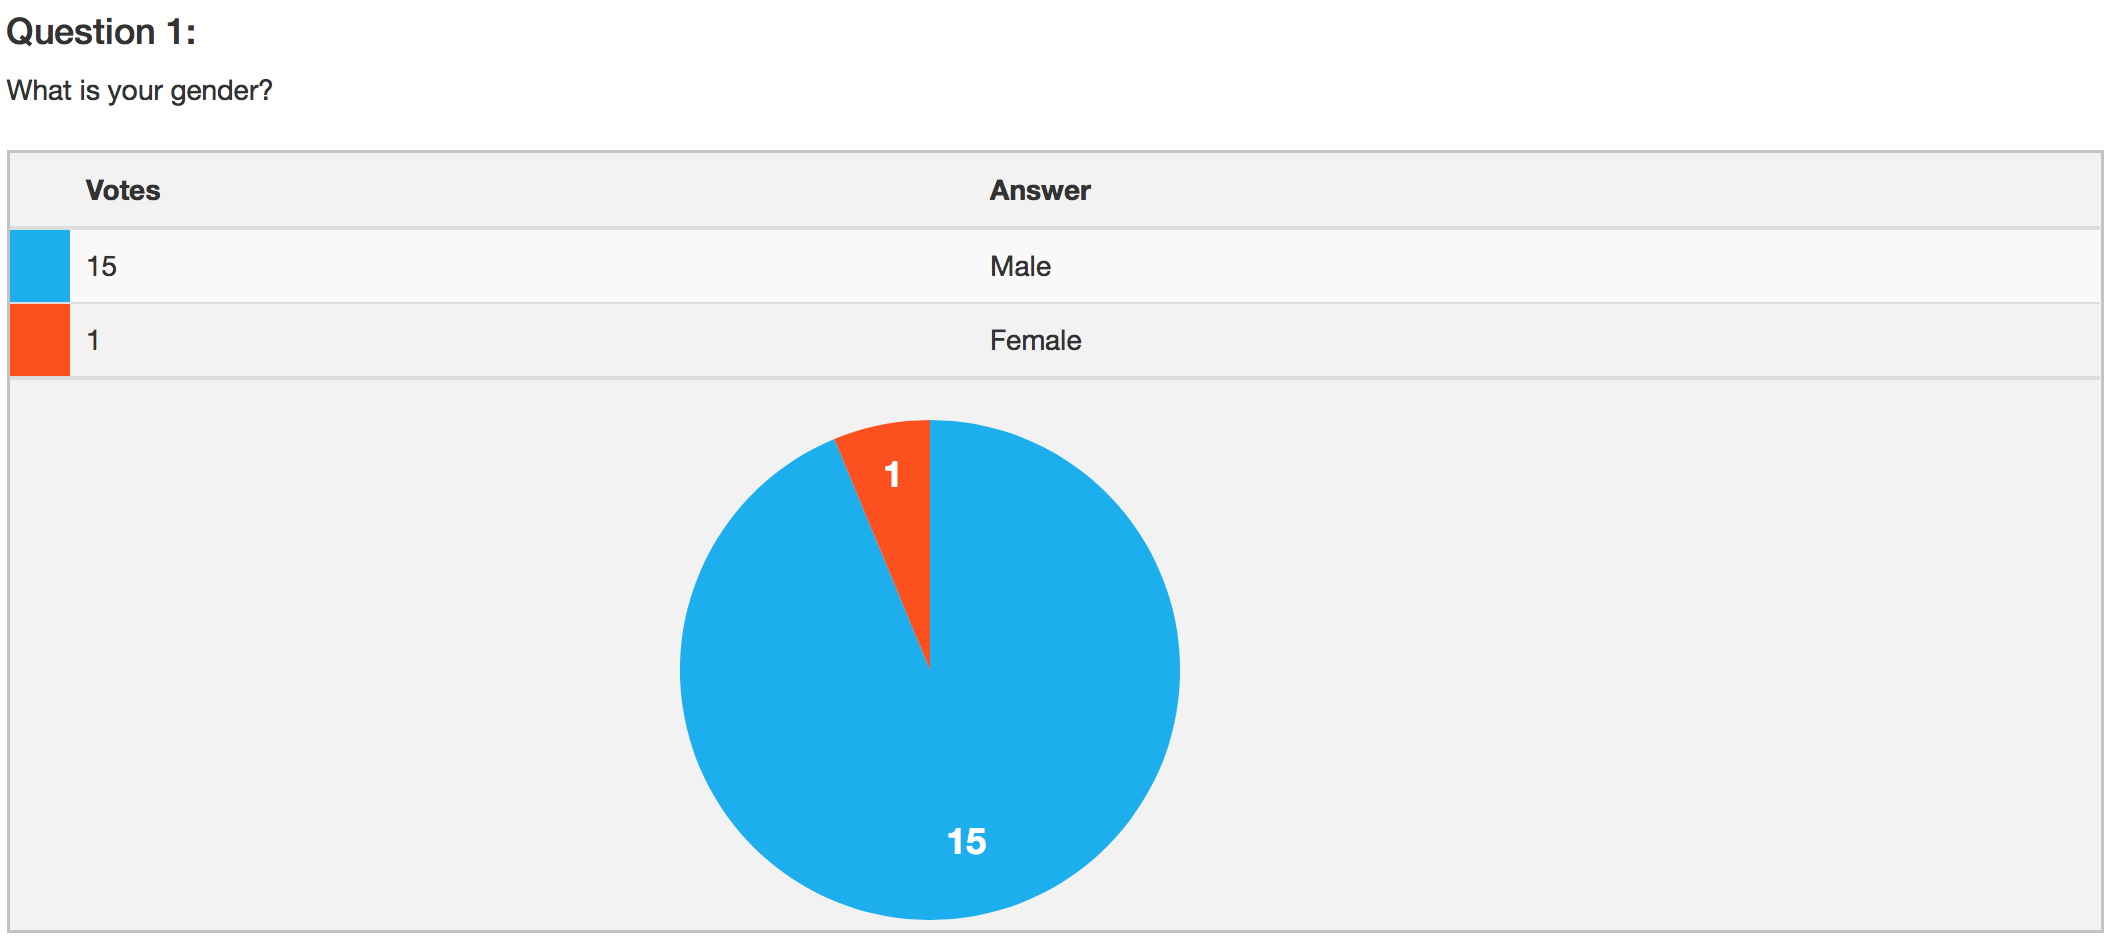
\includegraphics[width=14cm]{figures/votiee/w1q1}\\
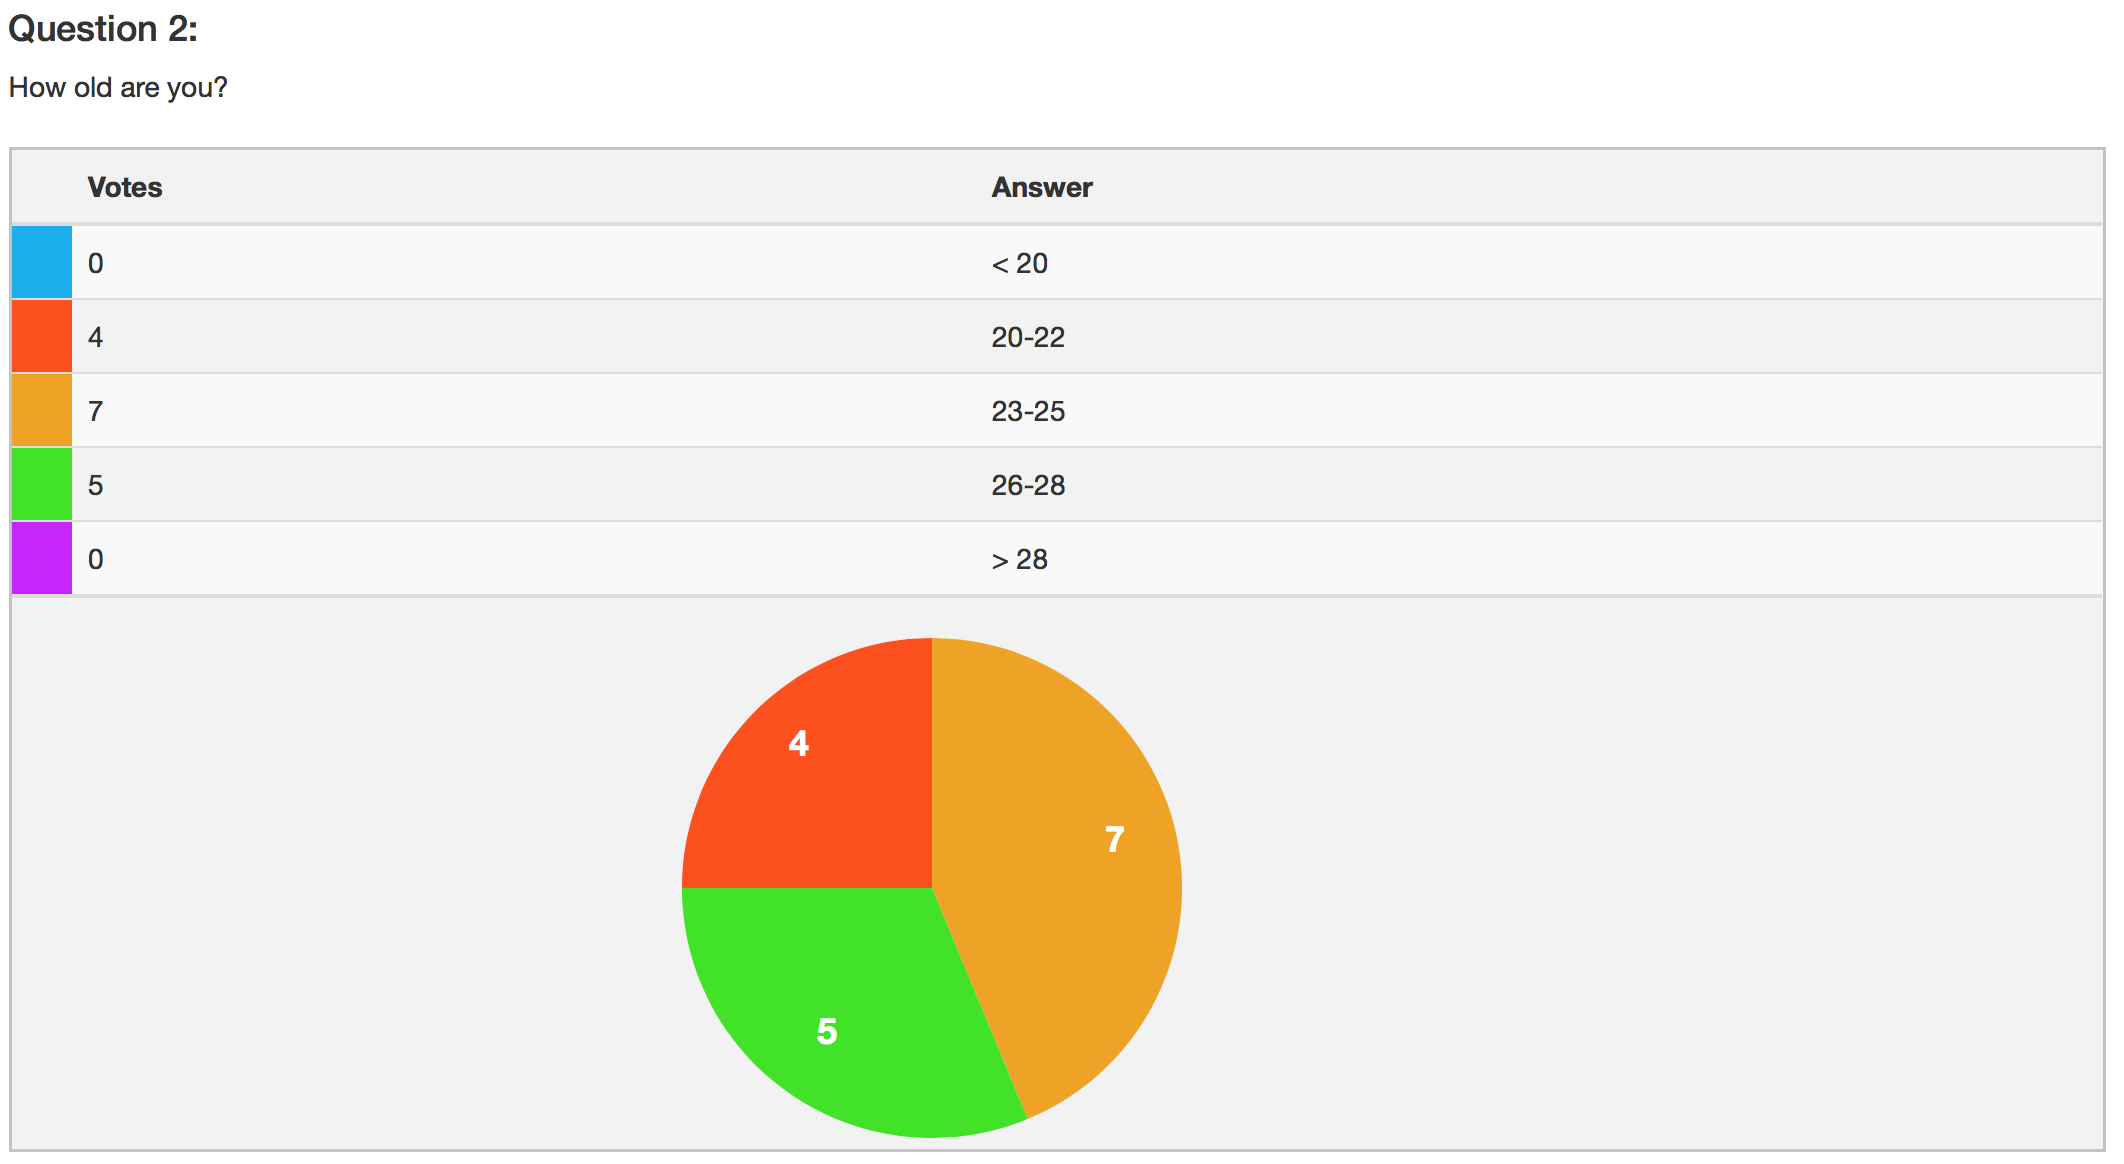
\includegraphics[width=14cm]{figures/votiee/w1q2}\\
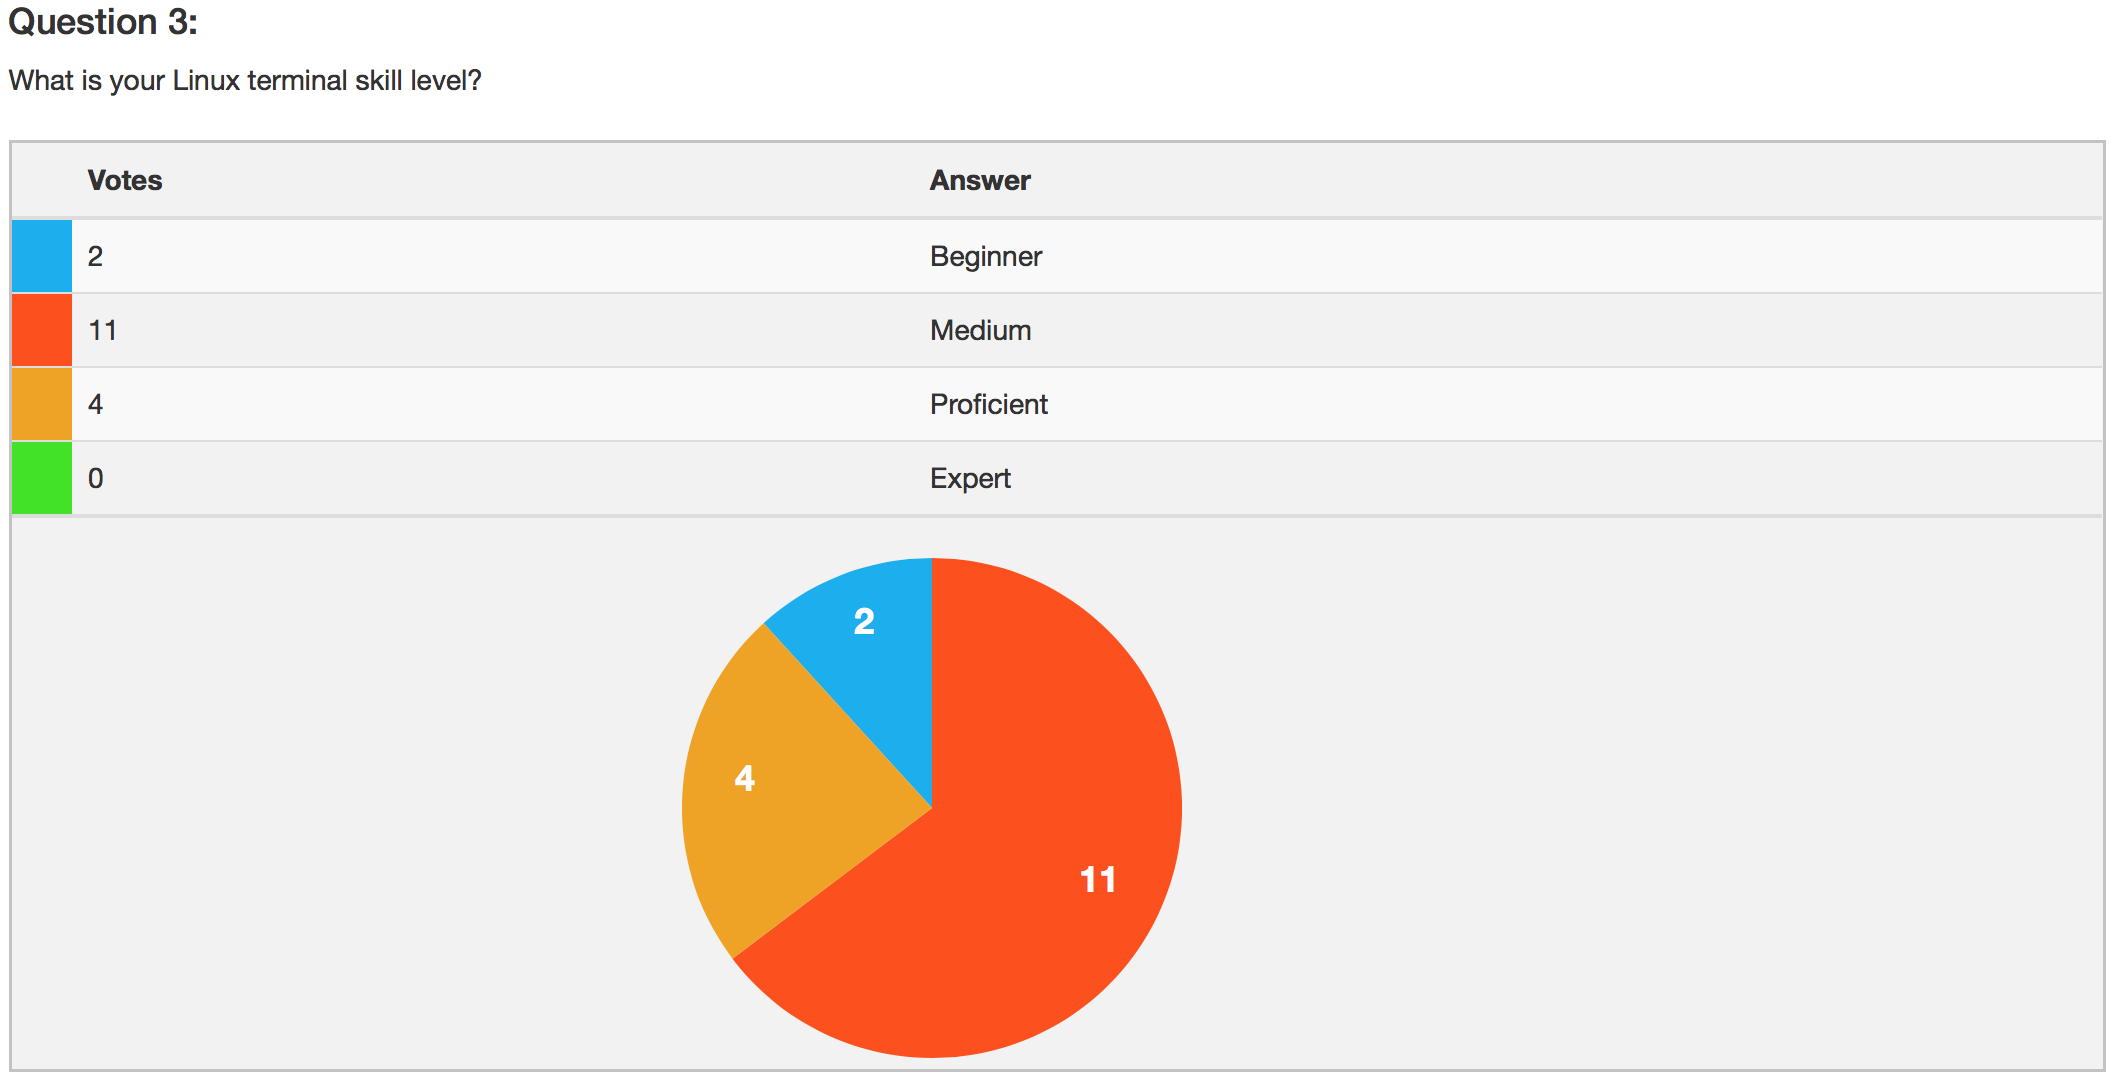
\includegraphics[width=14cm]{figures/votiee/w1q3}\\
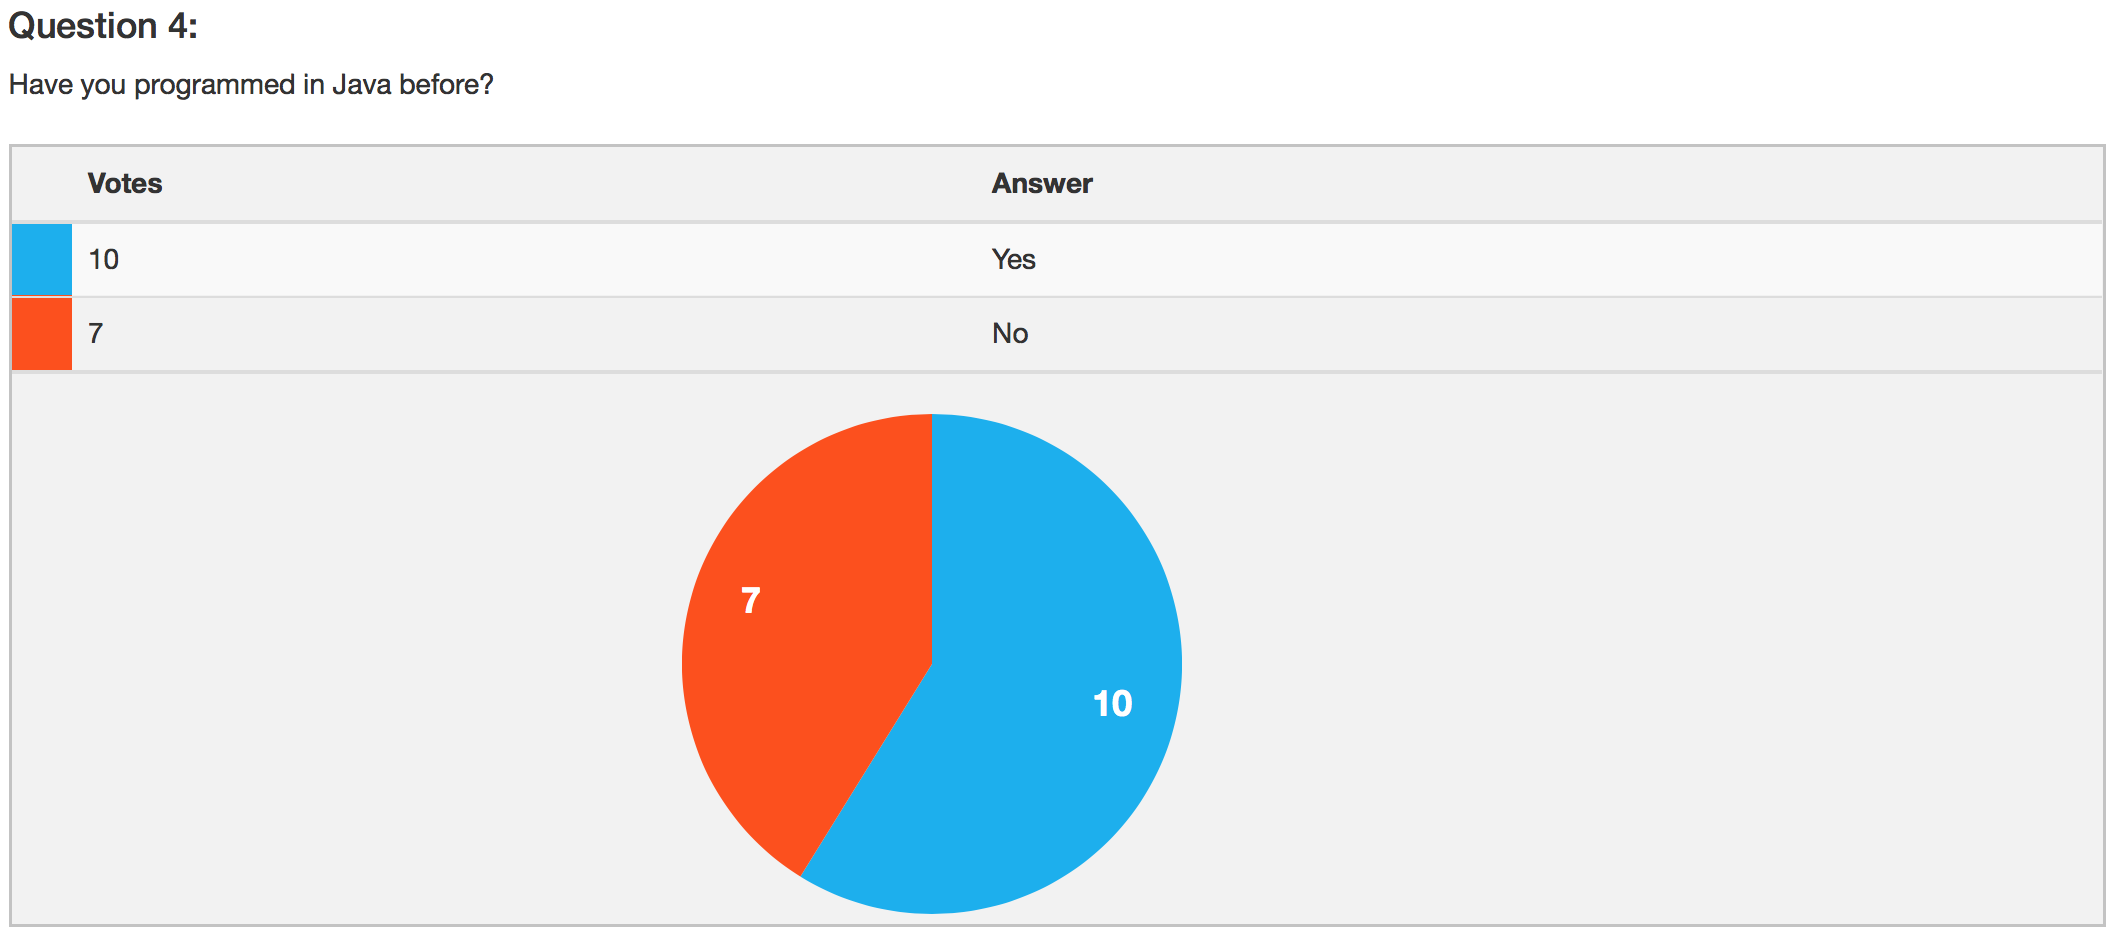
\includegraphics[width=14cm]{figures/votiee/w1q4}\\
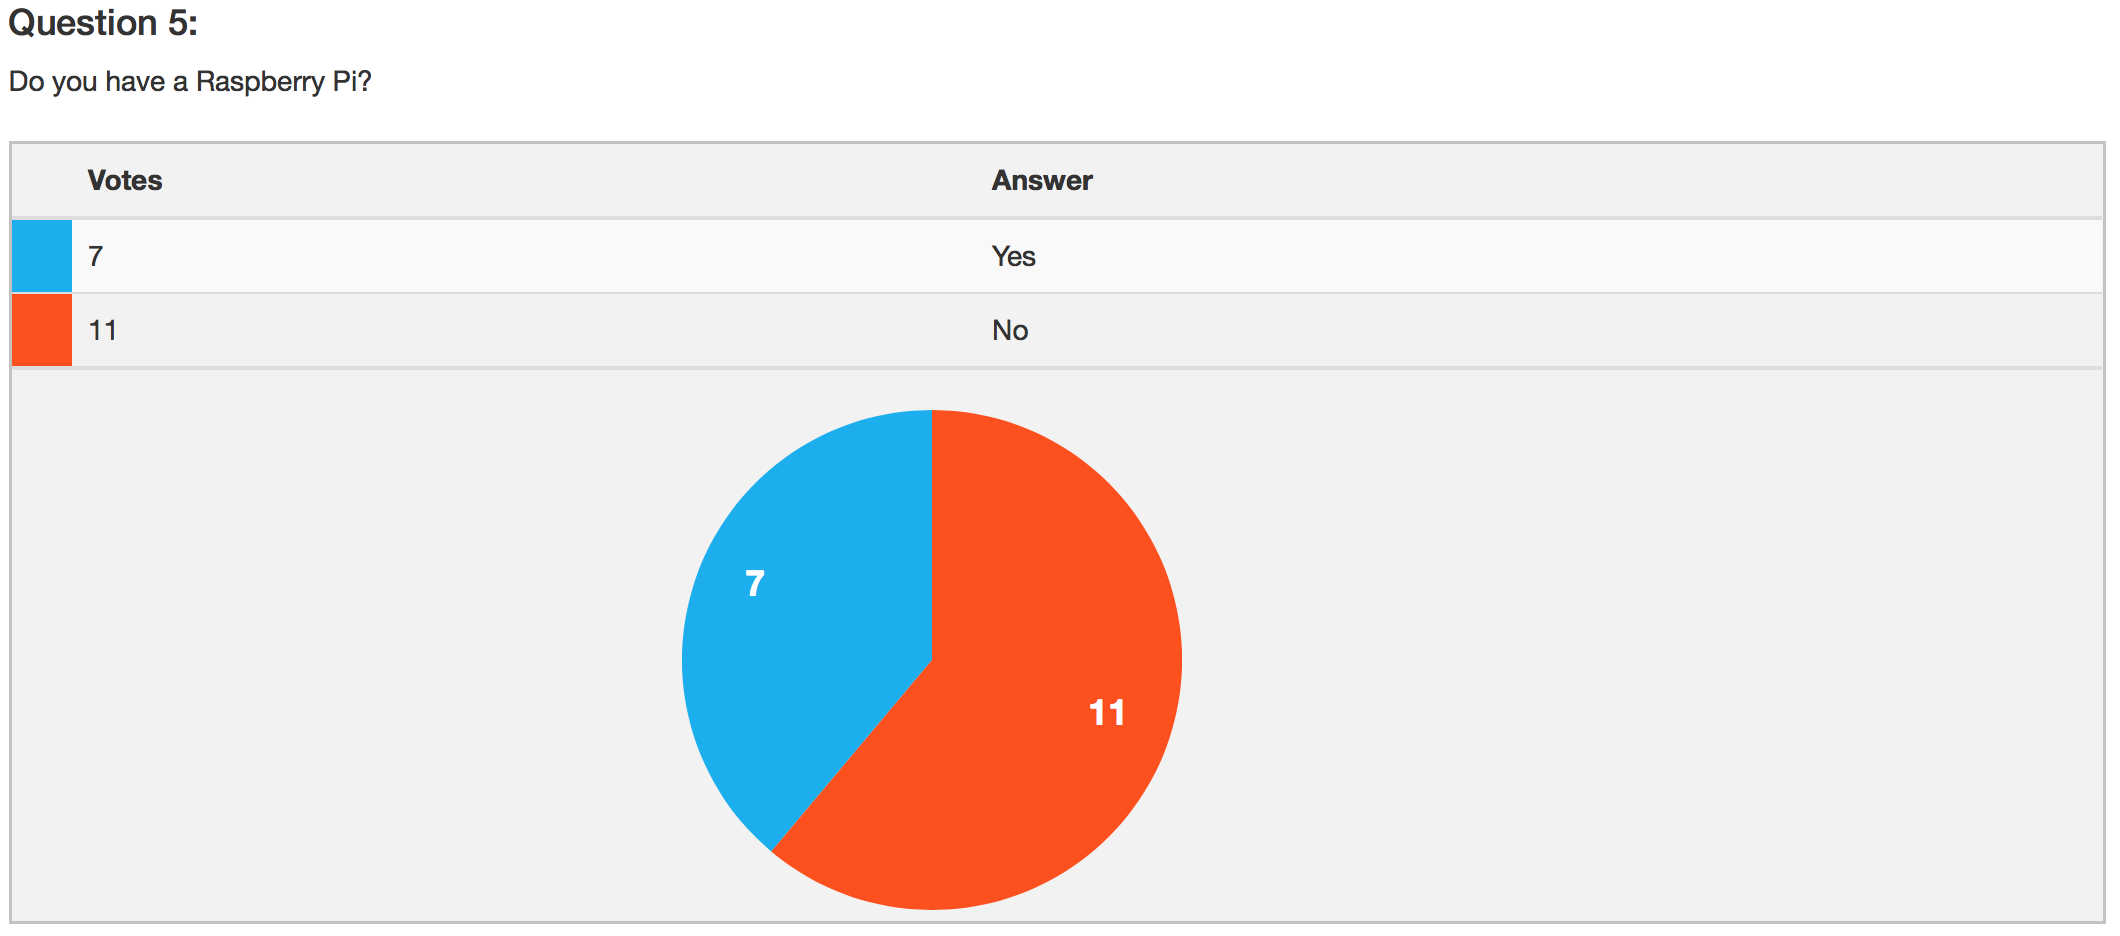
\includegraphics[width=14cm]{figures/votiee/w1q5}\\
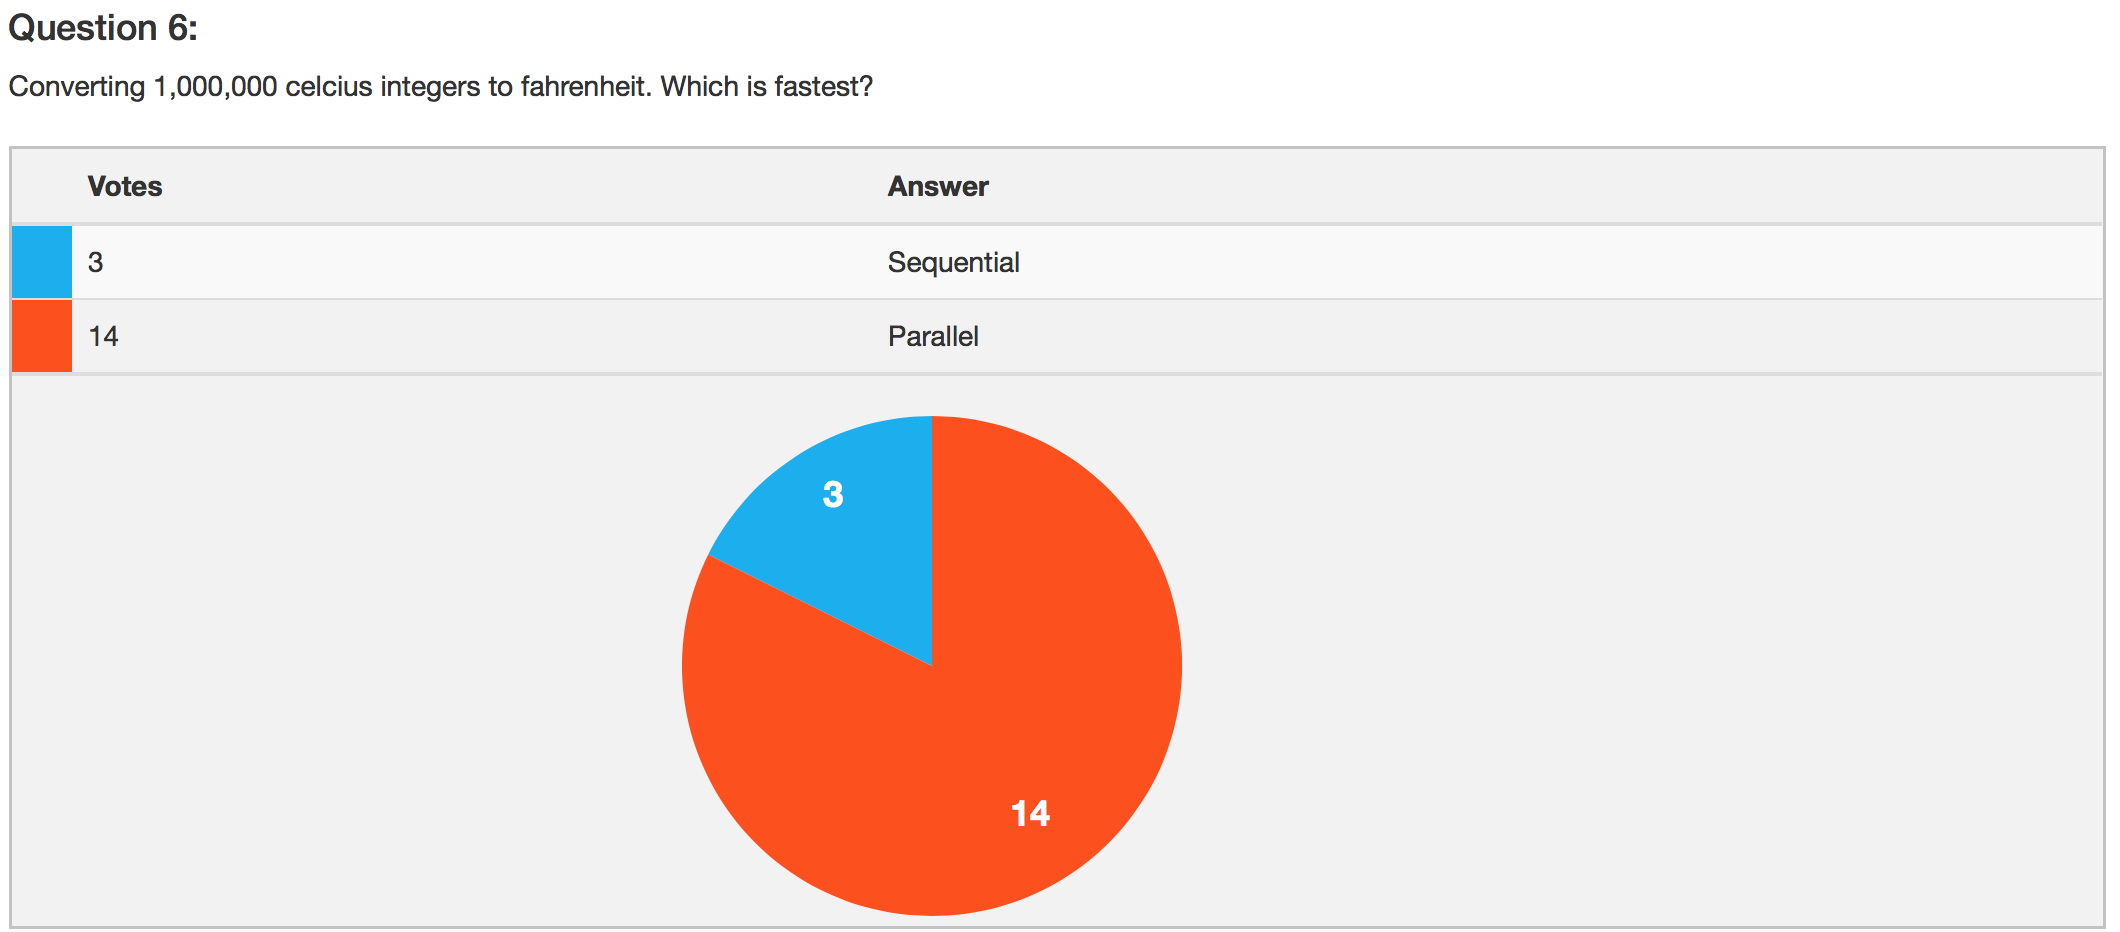
\includegraphics[width=14cm]{figures/votiee/w1q6}\\
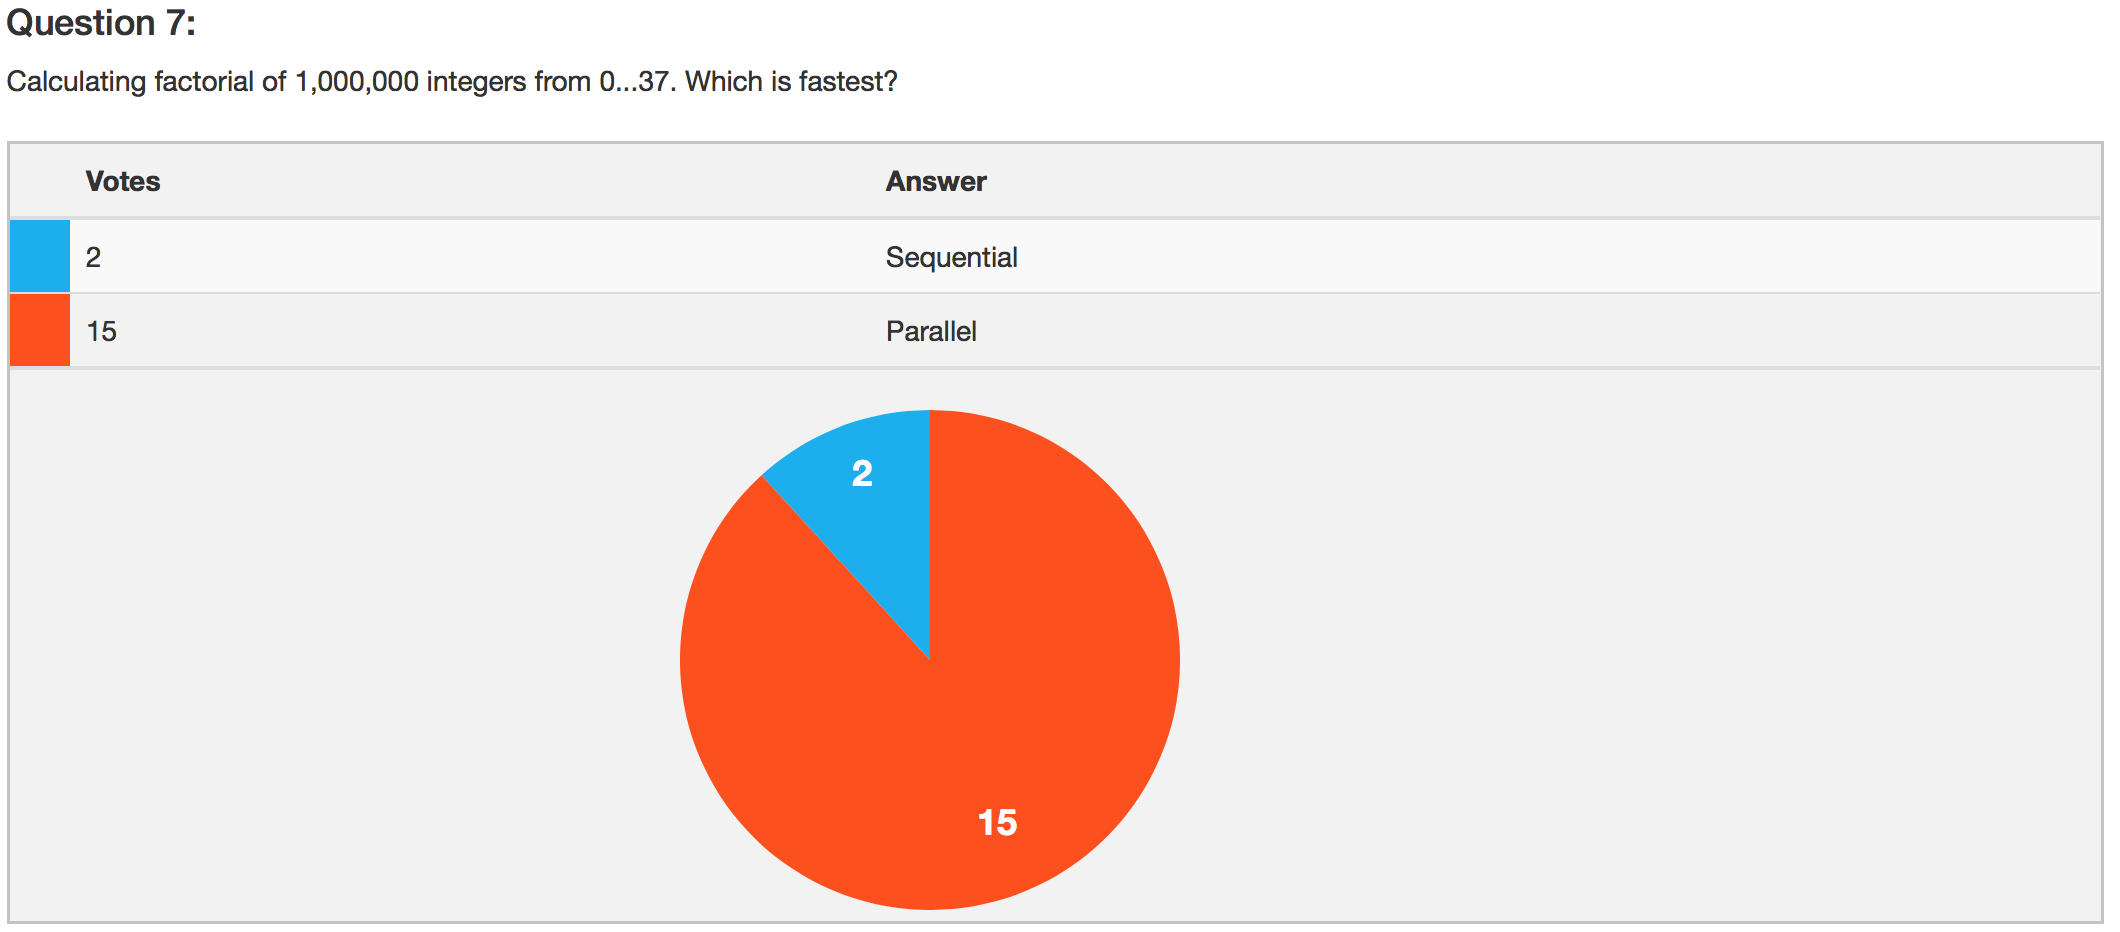
\includegraphics[width=14cm]{figures/votiee/w1q7}\\
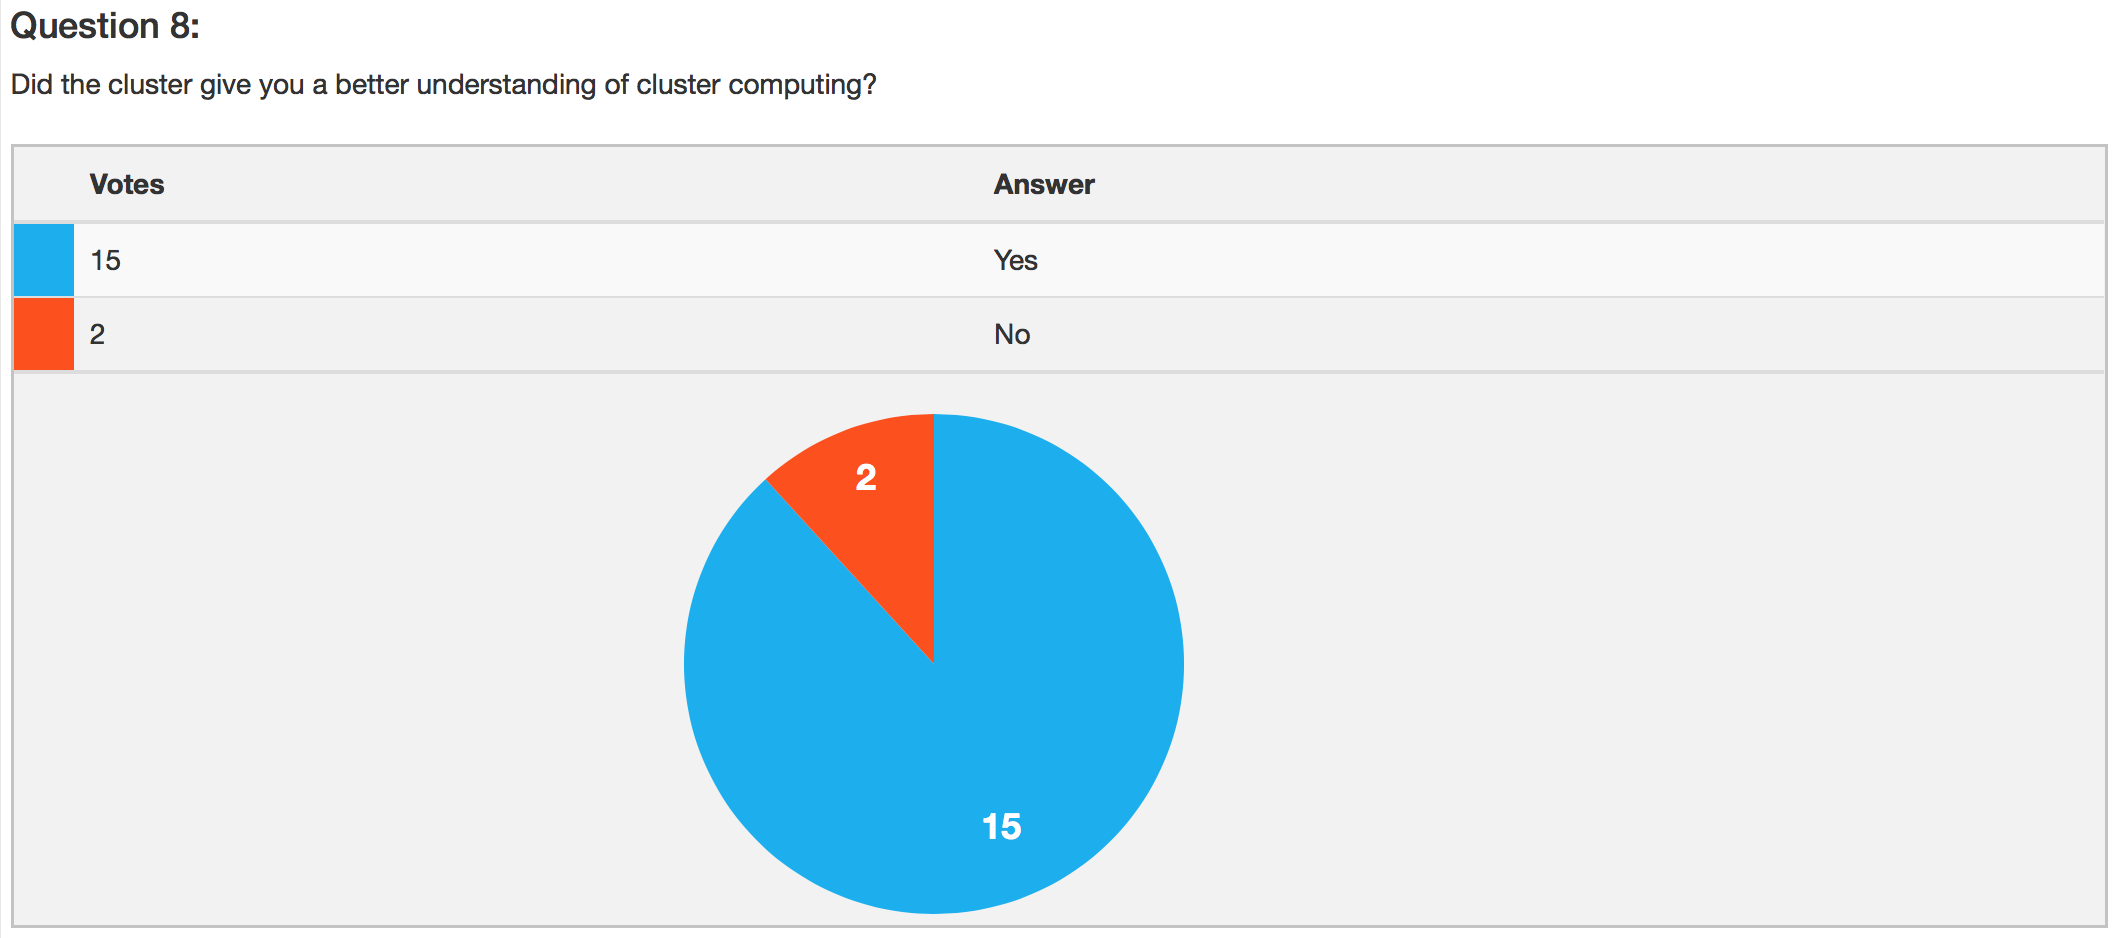
\includegraphics[width=14cm]{figures/votiee/w1q8}\\
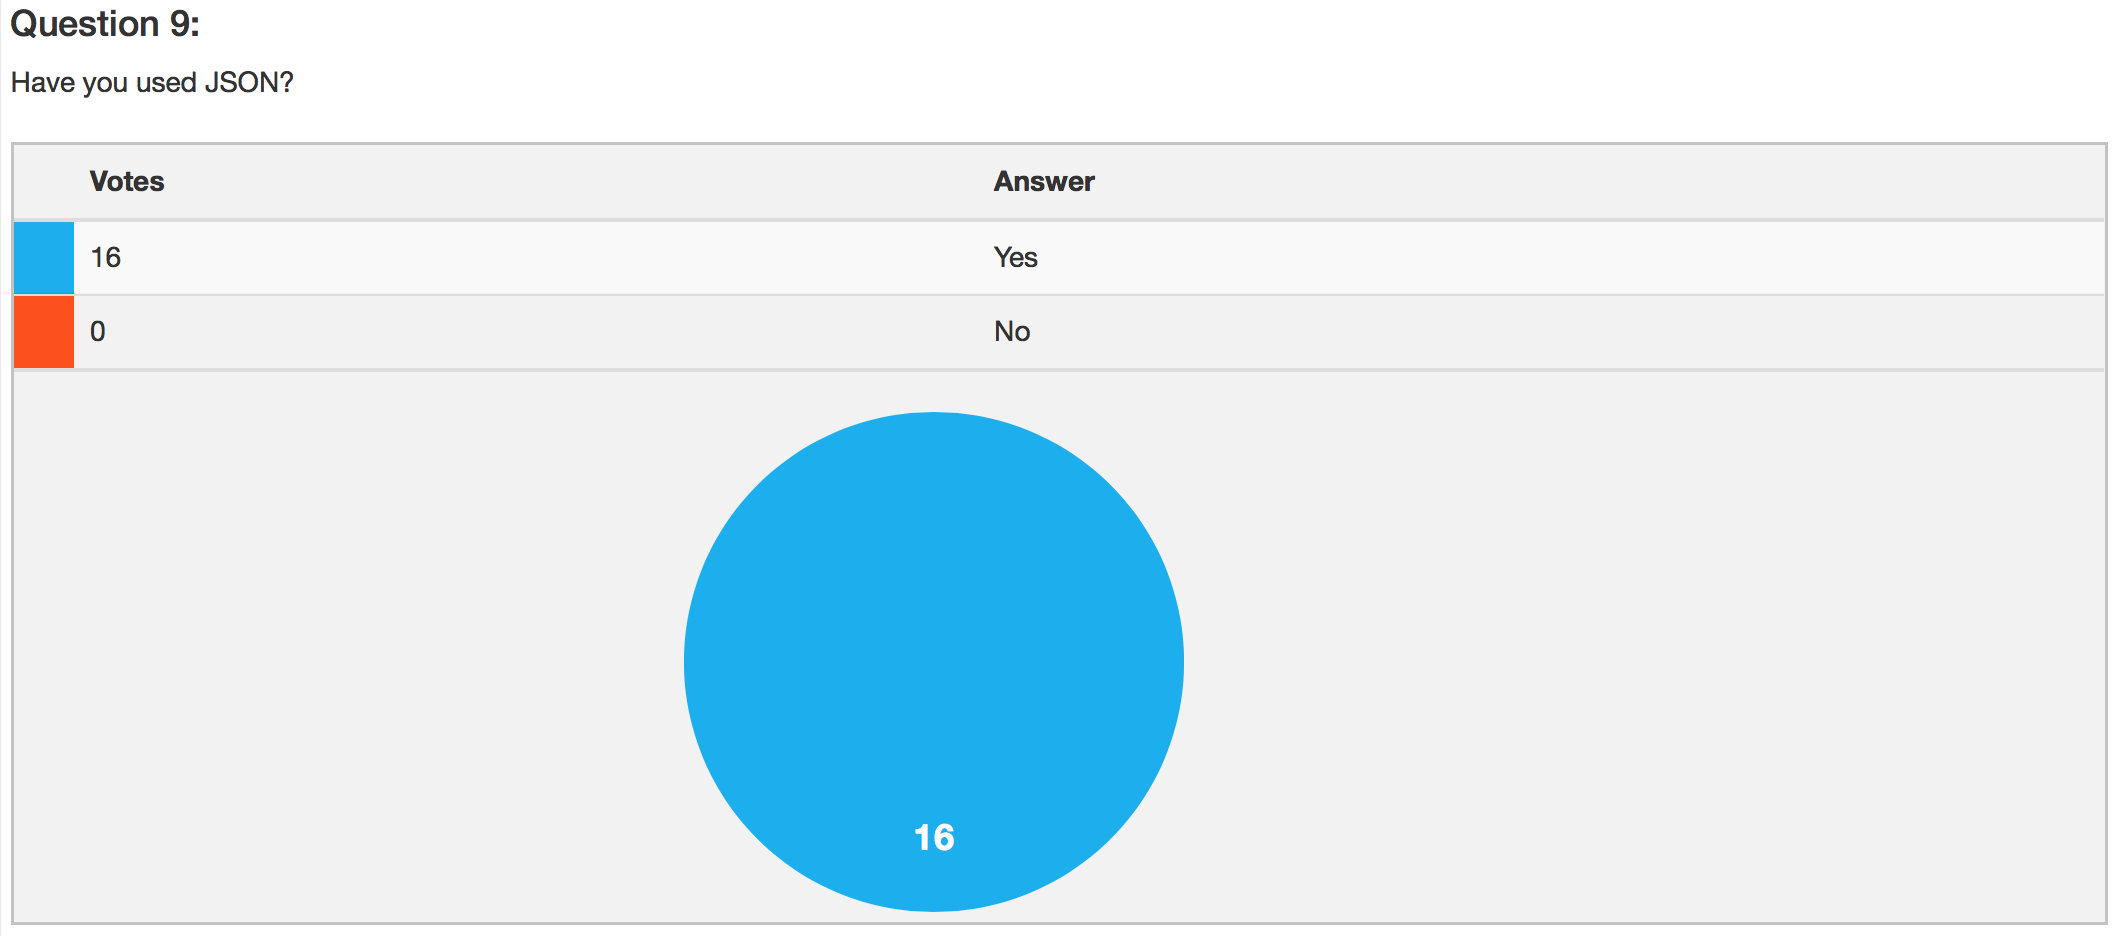
\includegraphics[width=14cm]{figures/votiee/w1q9}\\
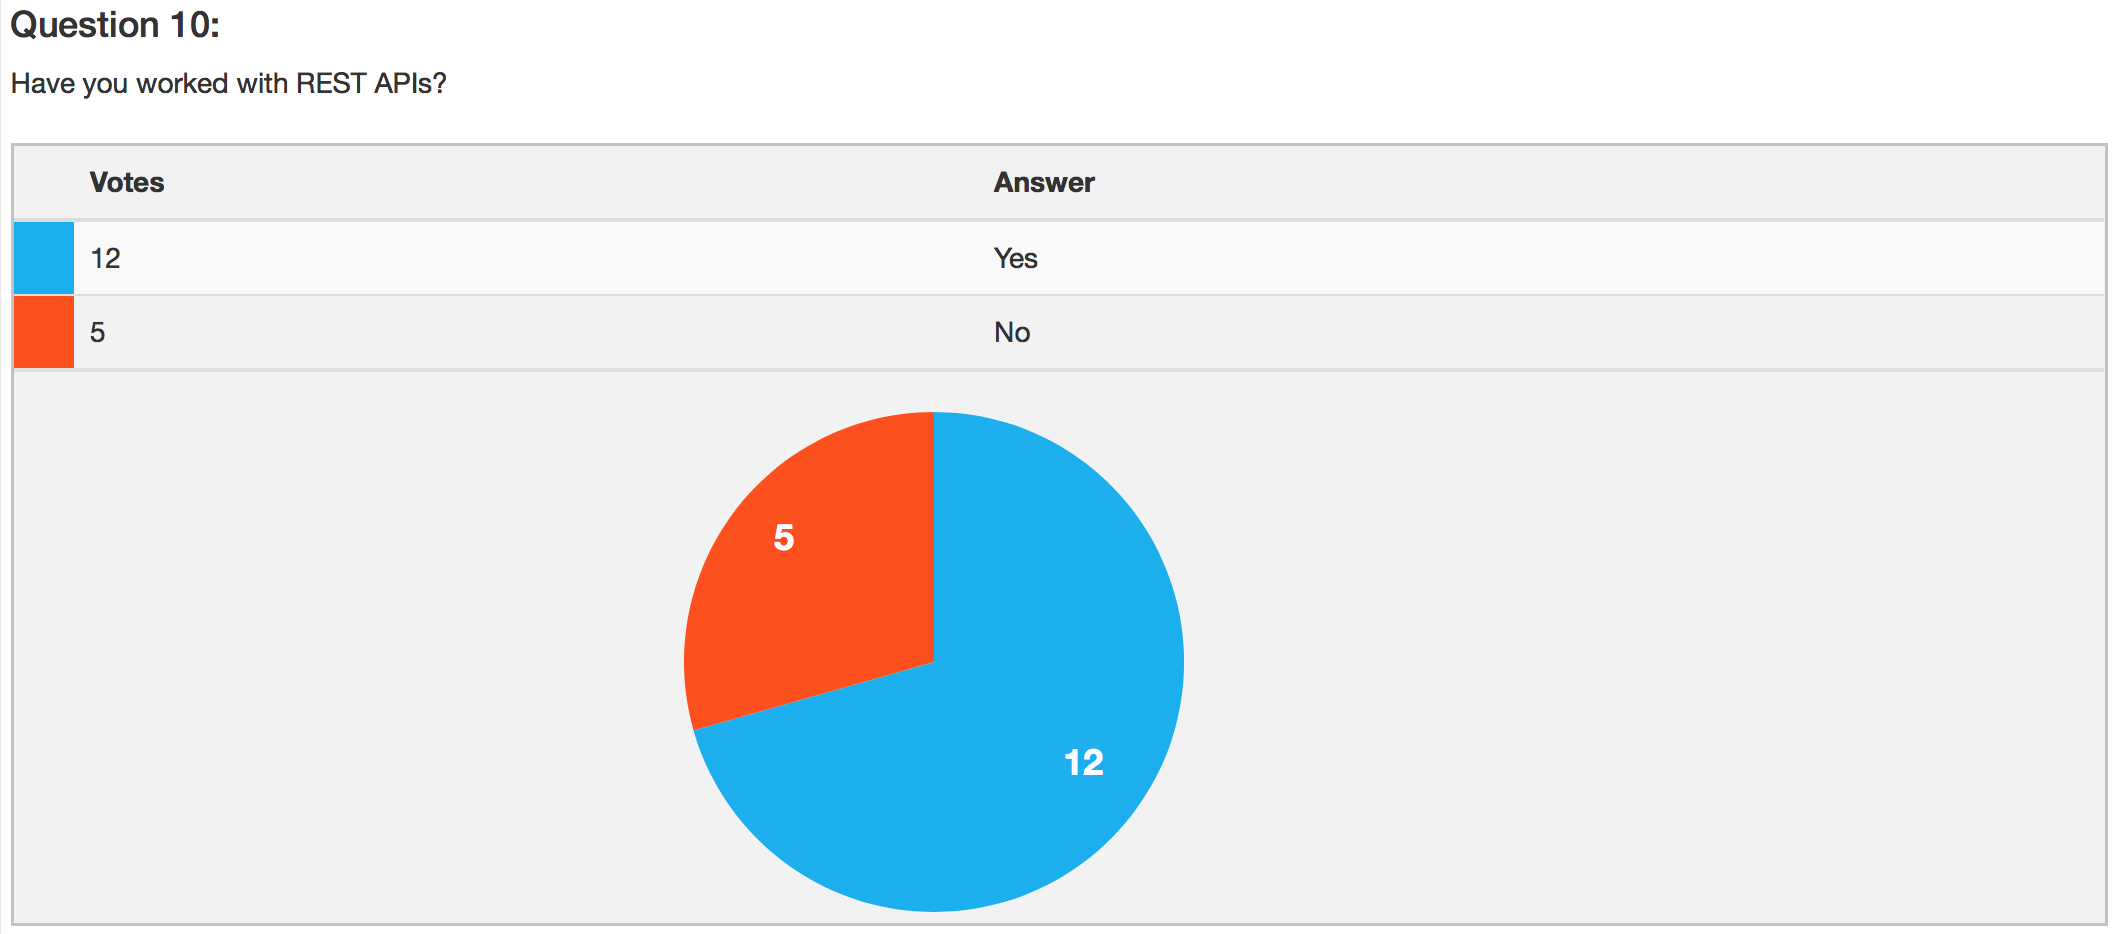
\includegraphics[width=14cm]{figures/votiee/w1q10}\\
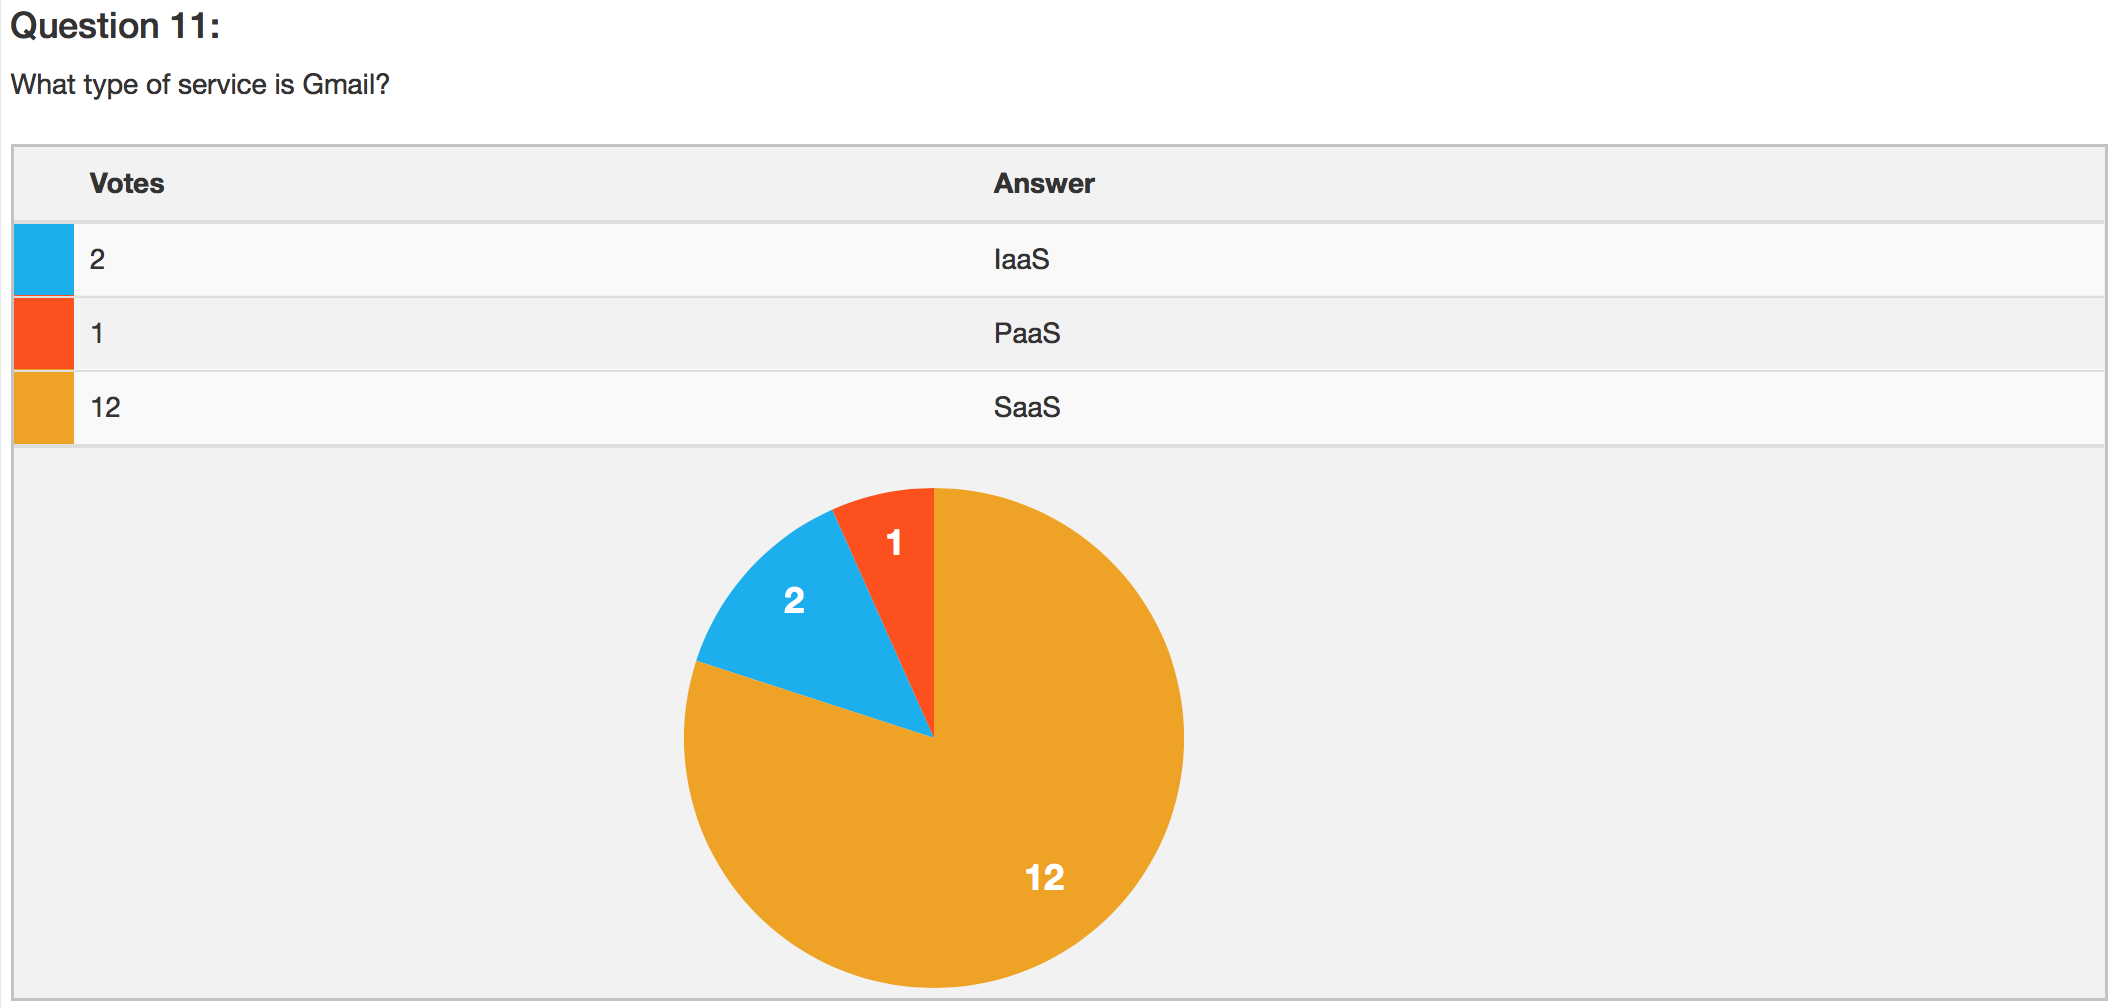
\includegraphics[width=14cm]{figures/votiee/w1q11}\\
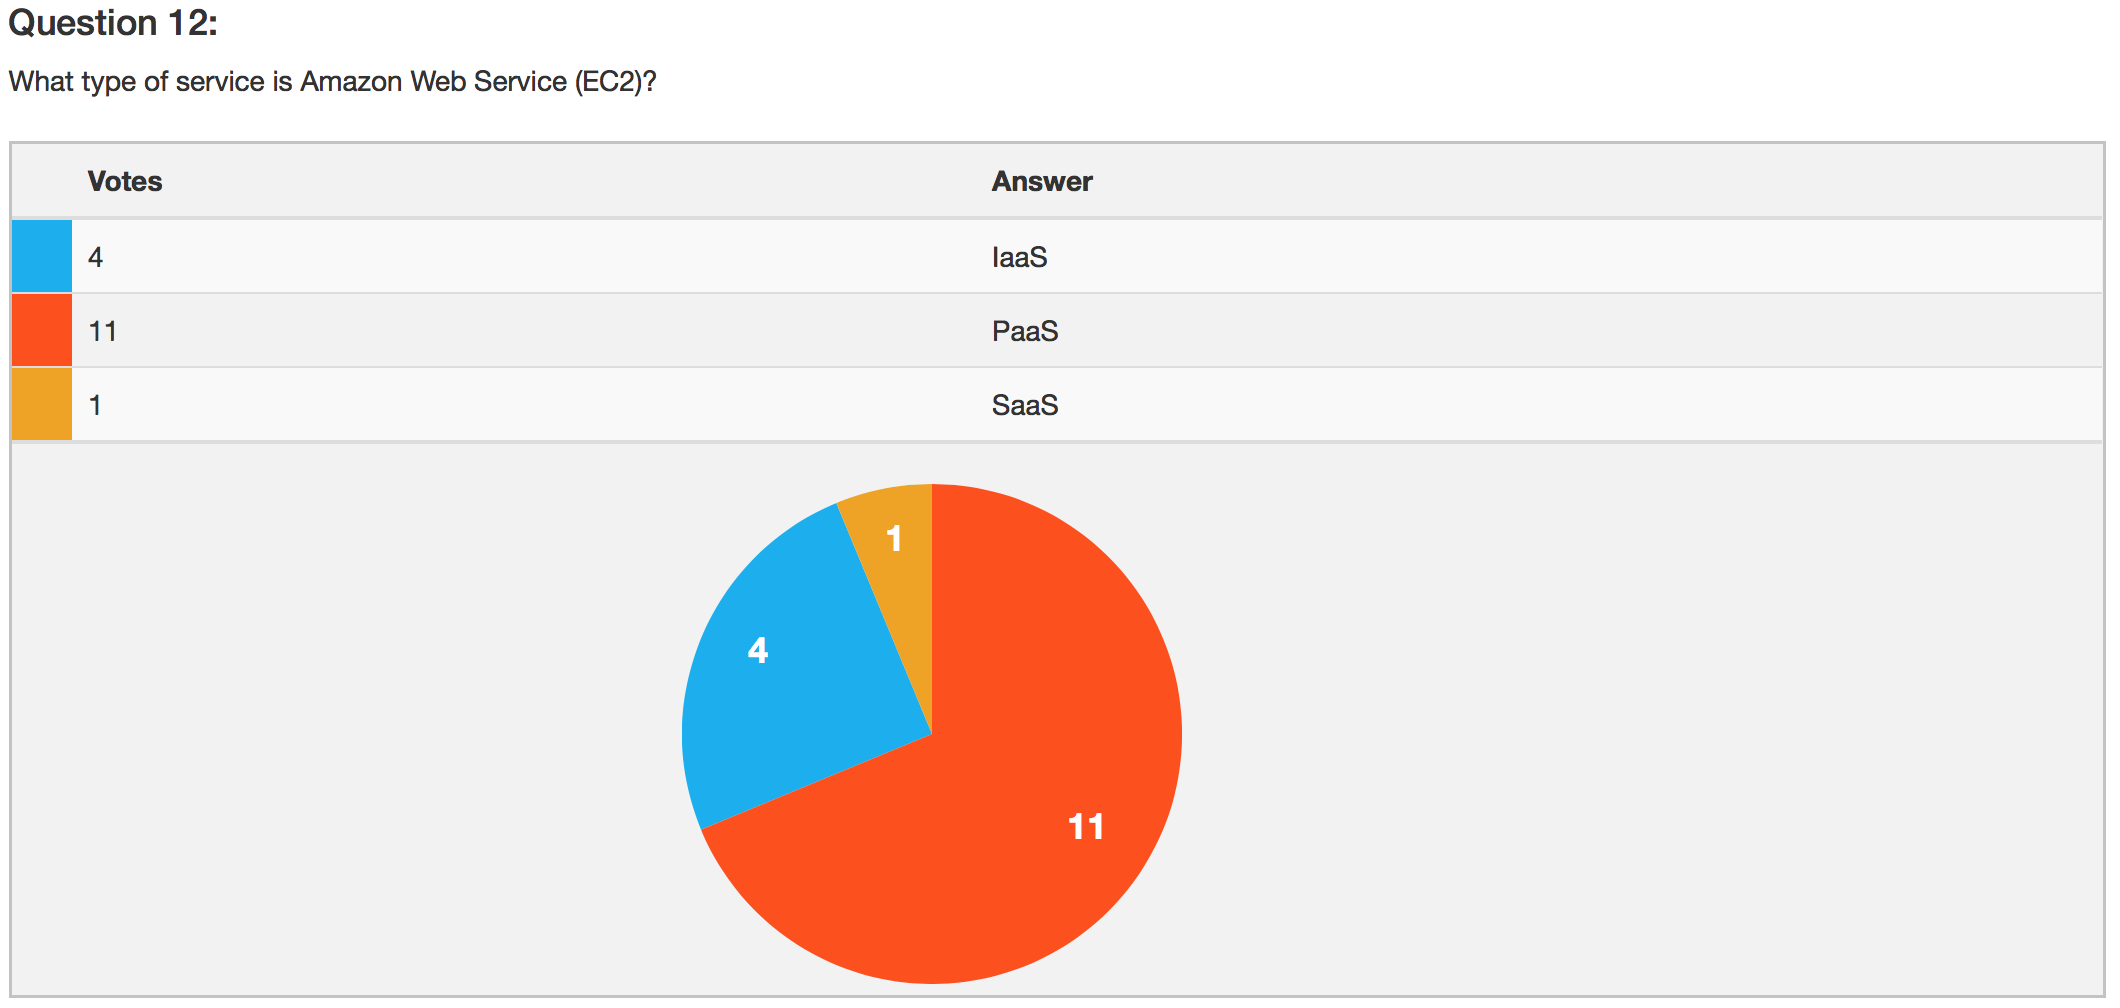
\includegraphics[width=14cm]{figures/votiee/w1q12}\\
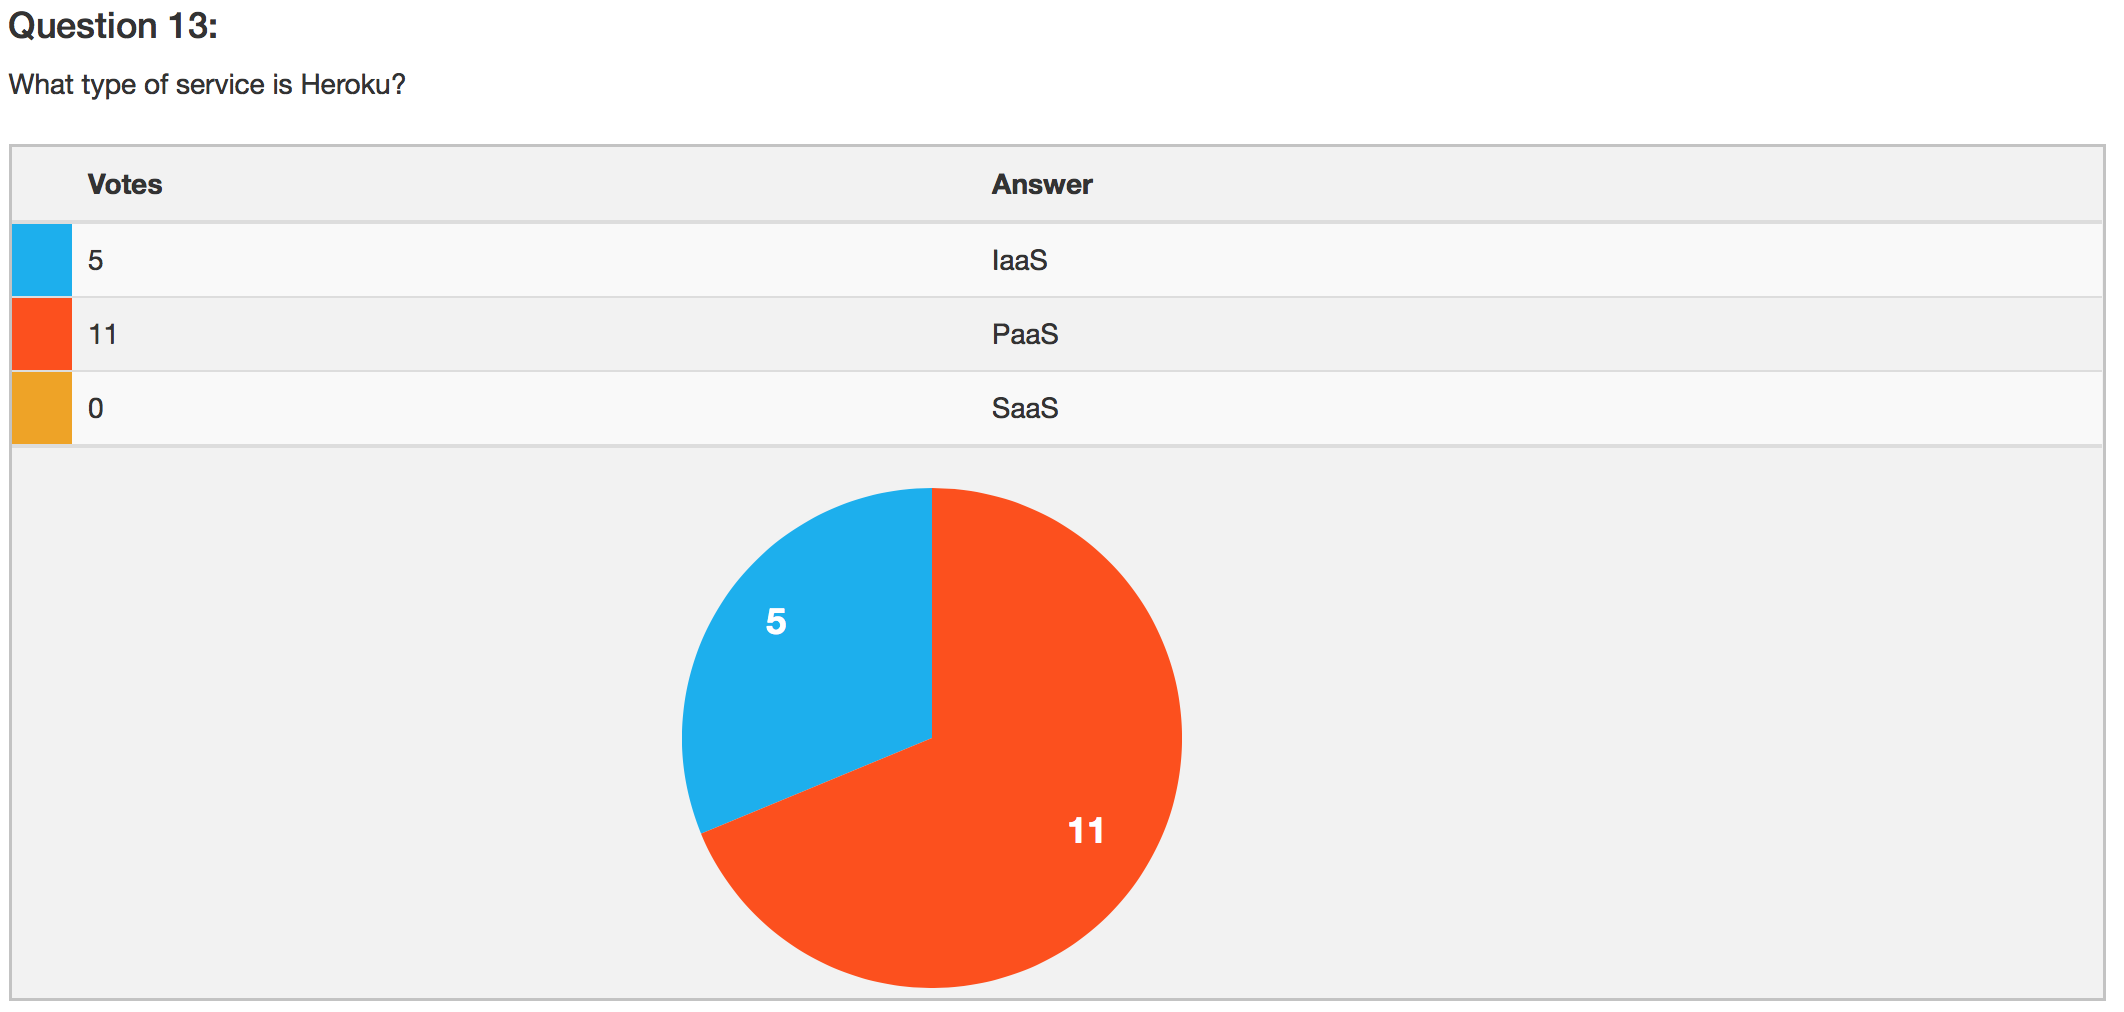
\includegraphics[width=14cm]{figures/votiee/w1q13}\\